


\begin{frame}
  \frametitle{In close collaboration with ... }

 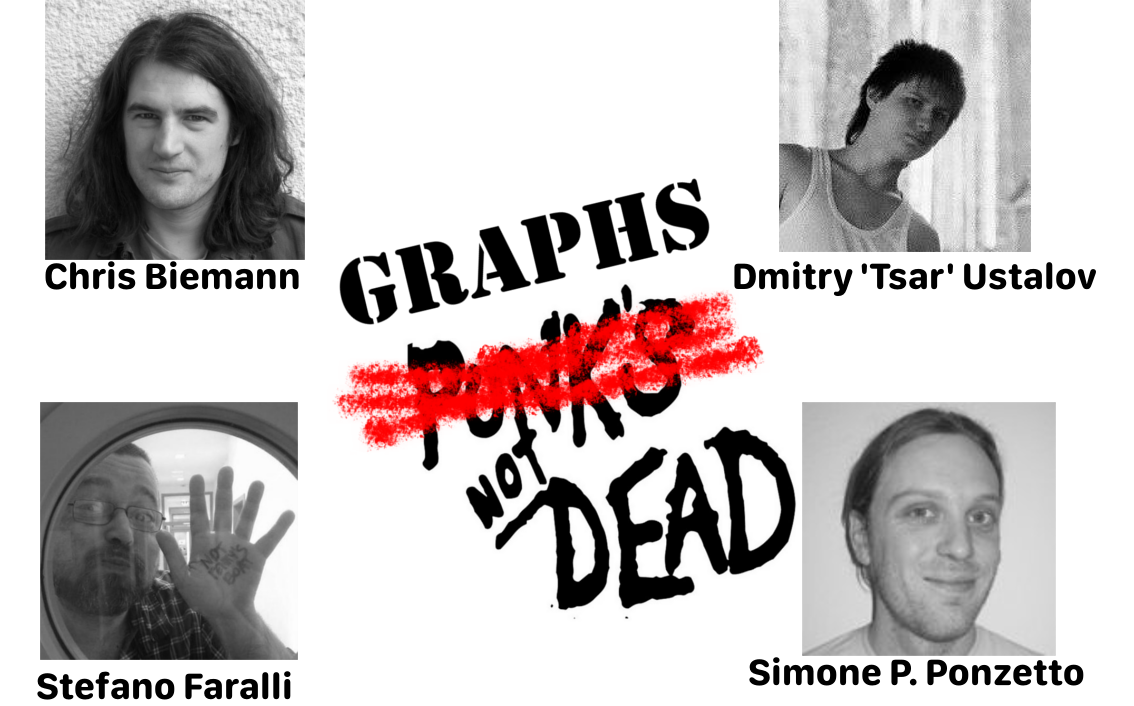
\includegraphics[width=.95\textwidth]{figures/collaborators}	
\end{frame}



\begin{frame}
  \frametitle{In collaboration with ... }
  { \large \bf
  \begin{itemize}
  	\item Andrei Kutuzov
  	\item Eugen Ruppert
  	\item Fide Marten
  	\item Nikolay Arefyev
  	\item Steffen Remus
  	\item Martin Riedl
  	\item Hubert Naets
   	\item Maria Pelevina
	\item Anastasiya Lopukhina
	\item Konstantin Lopukhin
  
  \end{itemize}	
  }
\end{frame}


\section{Motivation}



\begin{frame}{Deep Learning: everything is a vector}
	\vspace{-15pt}
	
  \begin{center}
  	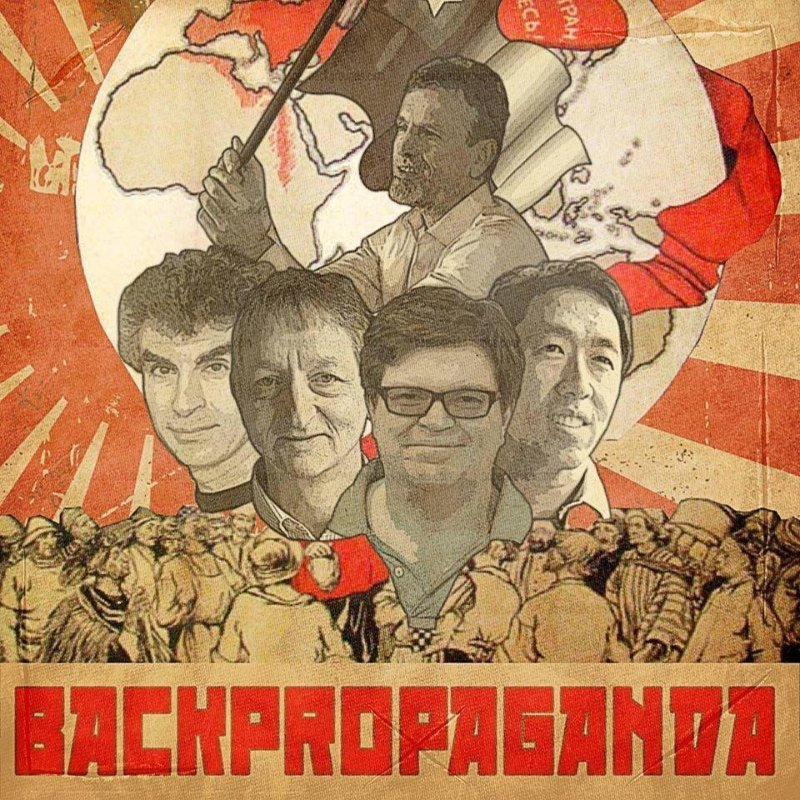
\includegraphics[width=0.59\textwidth]{figures/backprop}
  \end{center}
   
%{  \footnotesize
%  Image source: \url{https://www.linkedin.com/feed/update/urn:li:activity:6442811914803380224}
% } 

\end{frame}



\begin{frame}{Levels of Linguistic Analysis}
	\vspace{-15pt}
	
  \begin{center}
  	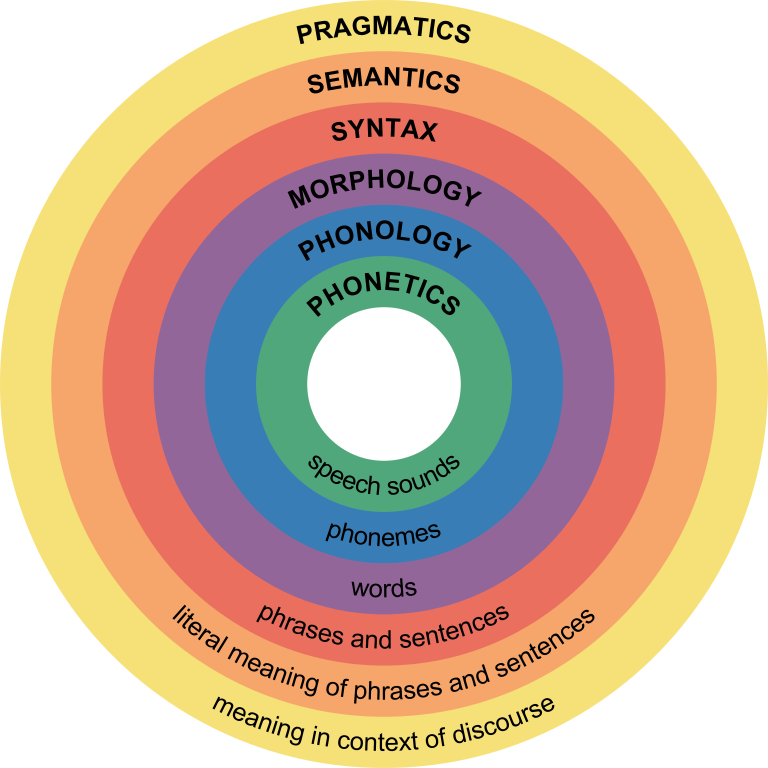
\includegraphics[width=0.59\textwidth]{figures/levels.svg}
  \end{center}
   
{  \footnotesize
  Image source: \url{https://commons.wikimedia.org/wiki/File:Major_levels_of_linguistic_structure.svg}
 } 

\end{frame}




\begin{frame}{Linguistic Structures and Graphs}
	
	\begin{itemize}
		\item (Written) language is a \alert{symbolic system}
	\end{itemize}	
	
\end{frame}


%
\begin{frame}{Graph Matrix Duality}
	\vspace{-25pt}
	
  \begin{center}
  	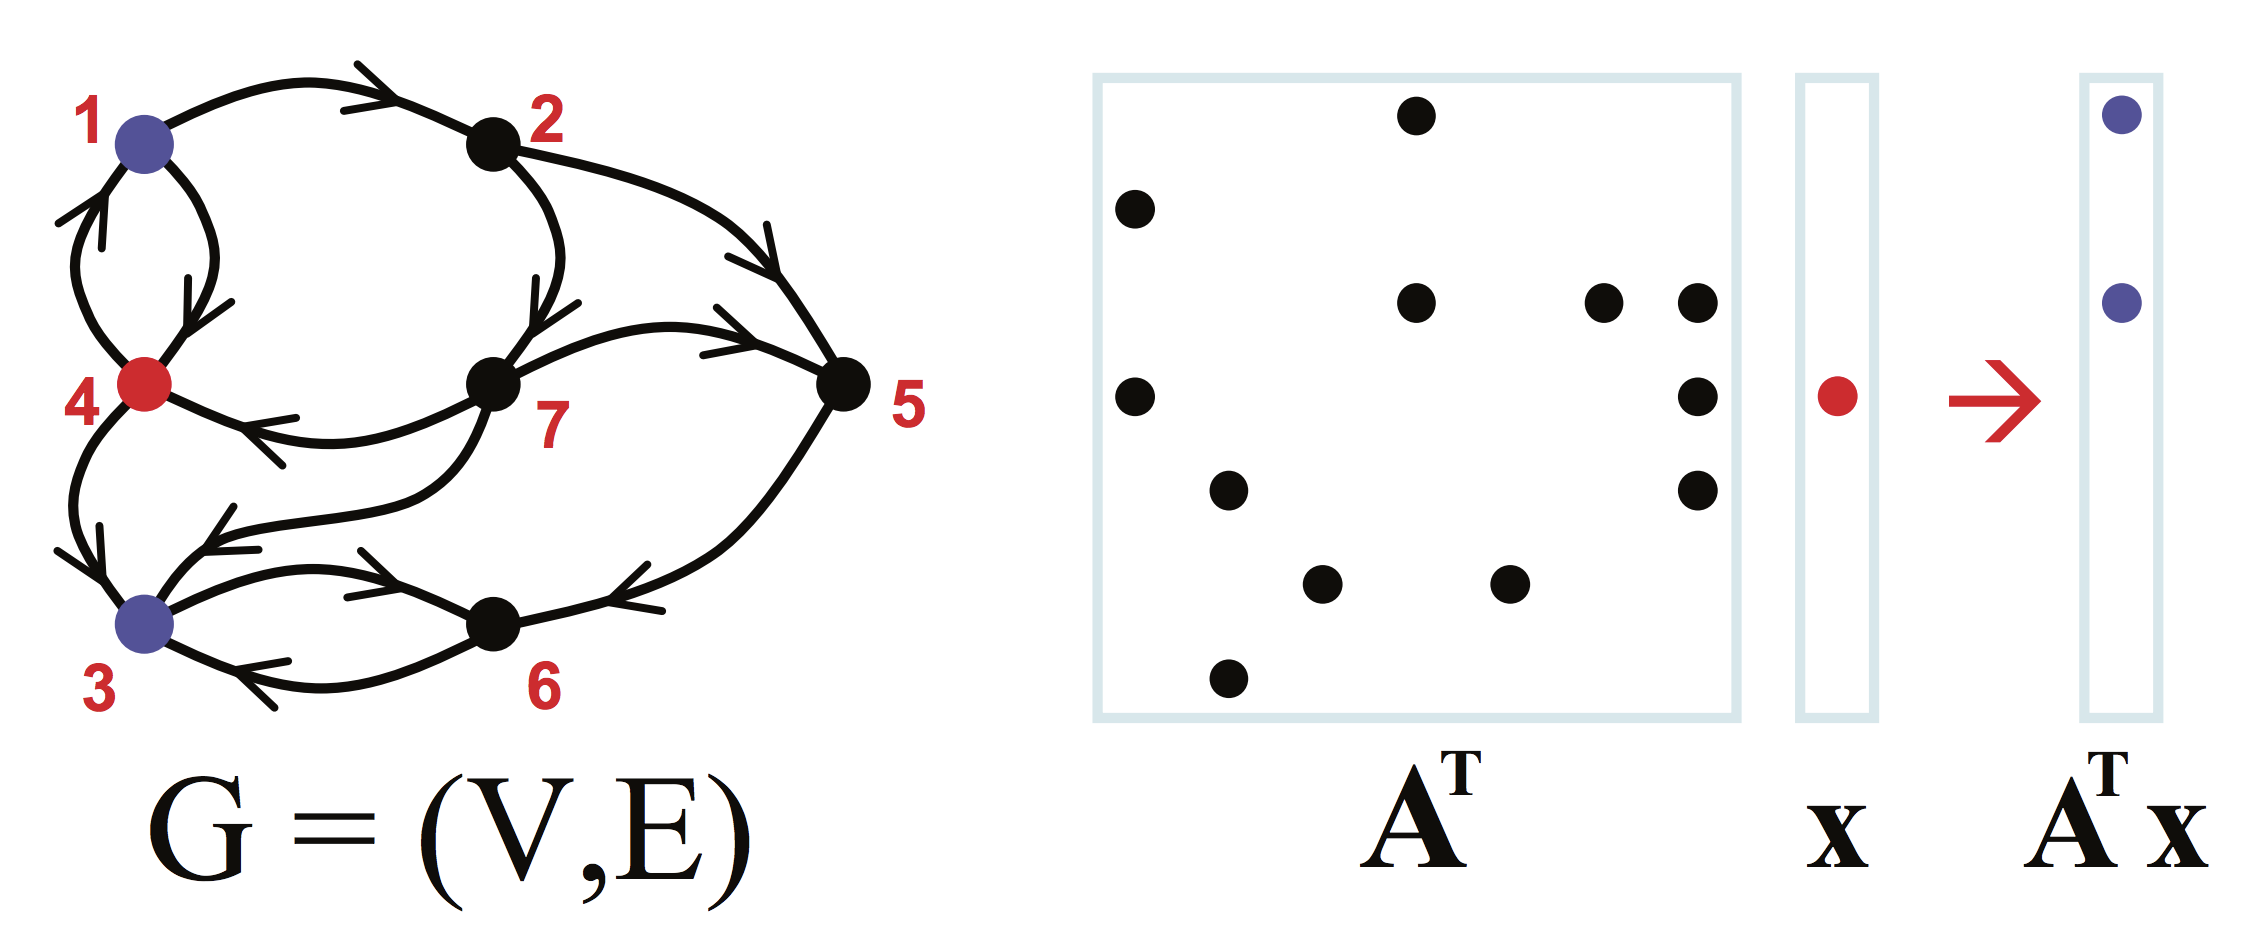
\includegraphics[width=0.99\textwidth]{figures/graph2matrix}
  \end{center}
  
  \pause 

  \begin{itemize}
  	\item   Adjacency matrix $\mathbf{A}$ is dual with the corresponding graph $G$.
  	\pause 
  	\item Vector matrix multiply $\mathbf{A}^T\mathbf{x}$ is dual with breadth-first search.
  \end{itemize}
% 
%{  \footnotesize
%  Image source: \cite{kepner2011graph}
% } 
%
\end{frame}


\begin{frame}{Goal}

  \begin{enumerate}
  	\item Learn the interpretable symbolic structures from text in an unsupervised way, which are \alert{more complex than tokens and lemmas}.
  	\pause 
  	\item Represent the learned structures in the vector form.
  	\pause 
  	\item Use the vector representations instead/in addition to word embedding the deep learning applications. 
  	\pause 
  	\item More complex structures could improve performance, but also provide better interpretability of the deep learning models. 
  	
  \end{enumerate}

\end{frame}
